\subsection{Session: Poster Session 1}

\subsubsection{MRI Banding Removal via Adversarial Training \cite{DefazioMR20}}

Talk by \textit{Aaron Defazio}. \\

{\bf Motivation:} even current SOTA reconstructions of cascades of U-Nets may produce horizontally aligned banding artefacts (fig. \ref{fig:banding_arts}). 
Presence of such artefacts can be a major roadblock towards deploying MR reconstruction systems in production. \\

\begin{figure}[h!]
    \centering
    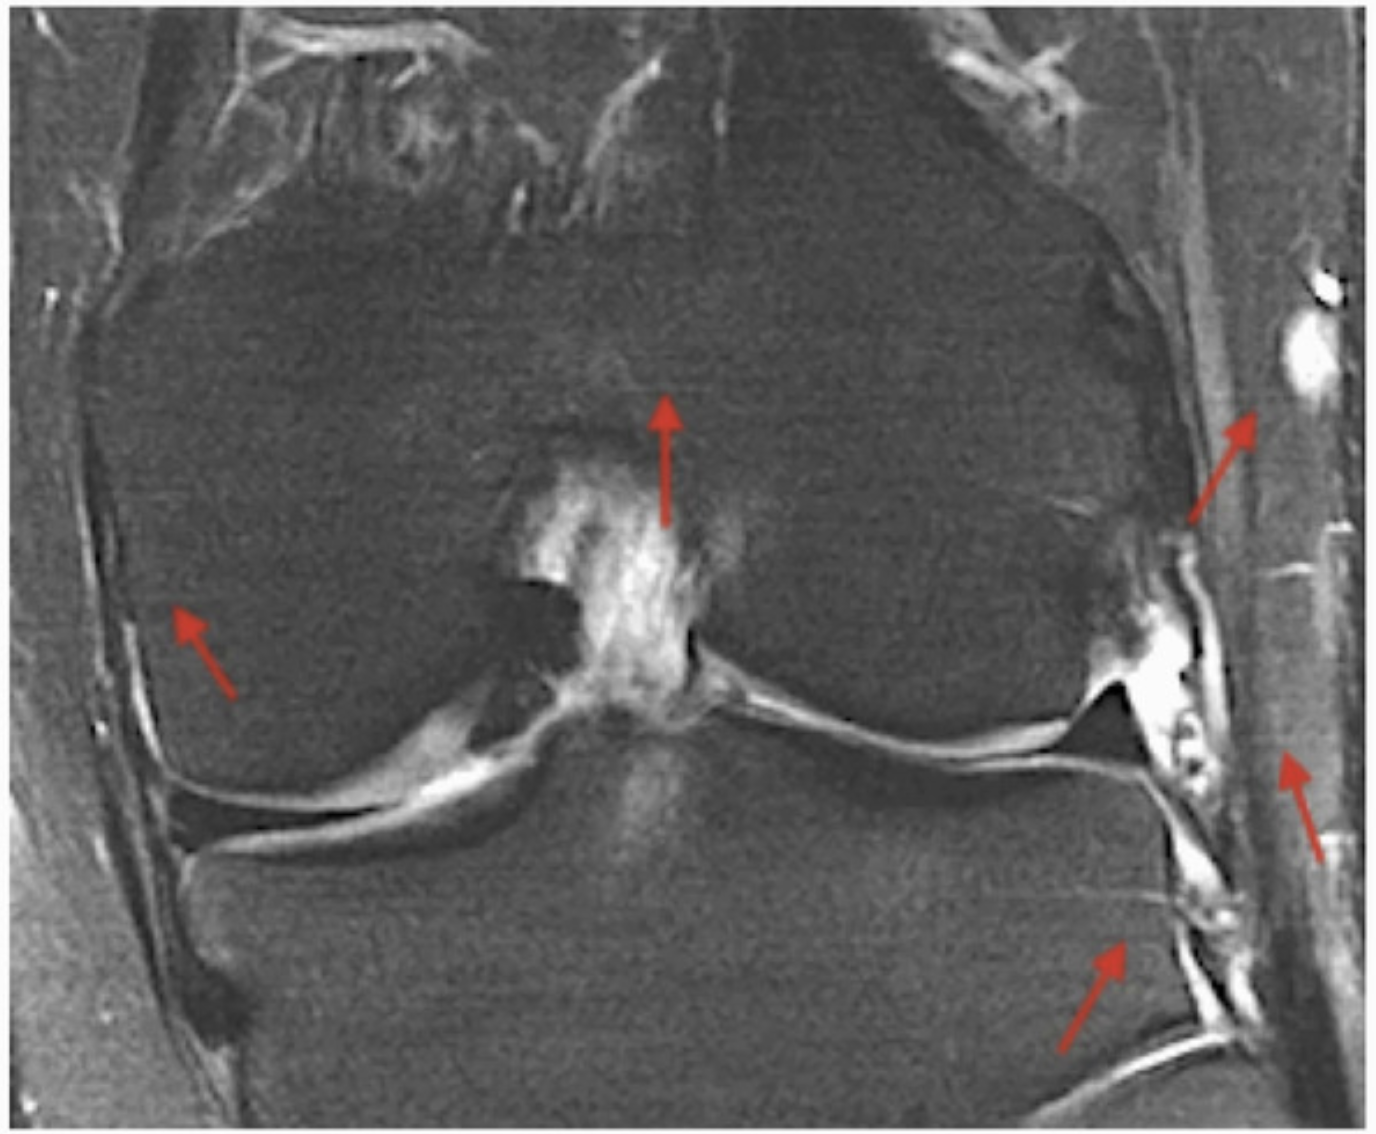
\includegraphics[scale=0.4]{neurips-2020/images/Screenshot 2020-12-15 at 09.25.34.png}
    \caption{Examples of banding artefacts presented on a reconstruction using "cascade of U-Nets" type of approach. Some of the artefacts are pointed with errors but actually they are everywhere on the image.}
    \label{fig:banding_arts}
\end{figure}

{\bf Note:} these artefacts are particularly evident for scans taken with 1.5T machines due to their additional noise. \\

{\bf Observation:} the direction striking artefacts is aligned with the direction of Cartesian undersampling. Hence if undersampling direction is changed by 90 degrees, horizontal artefacts will turn into vertical ones. \\

{\bf Method:} the full pipeline in presented on fig. \ref{fig:adversaria_art_removal_pipeline}. The main idea is to train a model with an adversarial component, where the discriminator network will distinguish between different directions of artefacts. 
For that, k-space can be transposed during the data preparation process (while the orientation of the image is preserved). \\

\begin{figure}[h!]
    \centering
    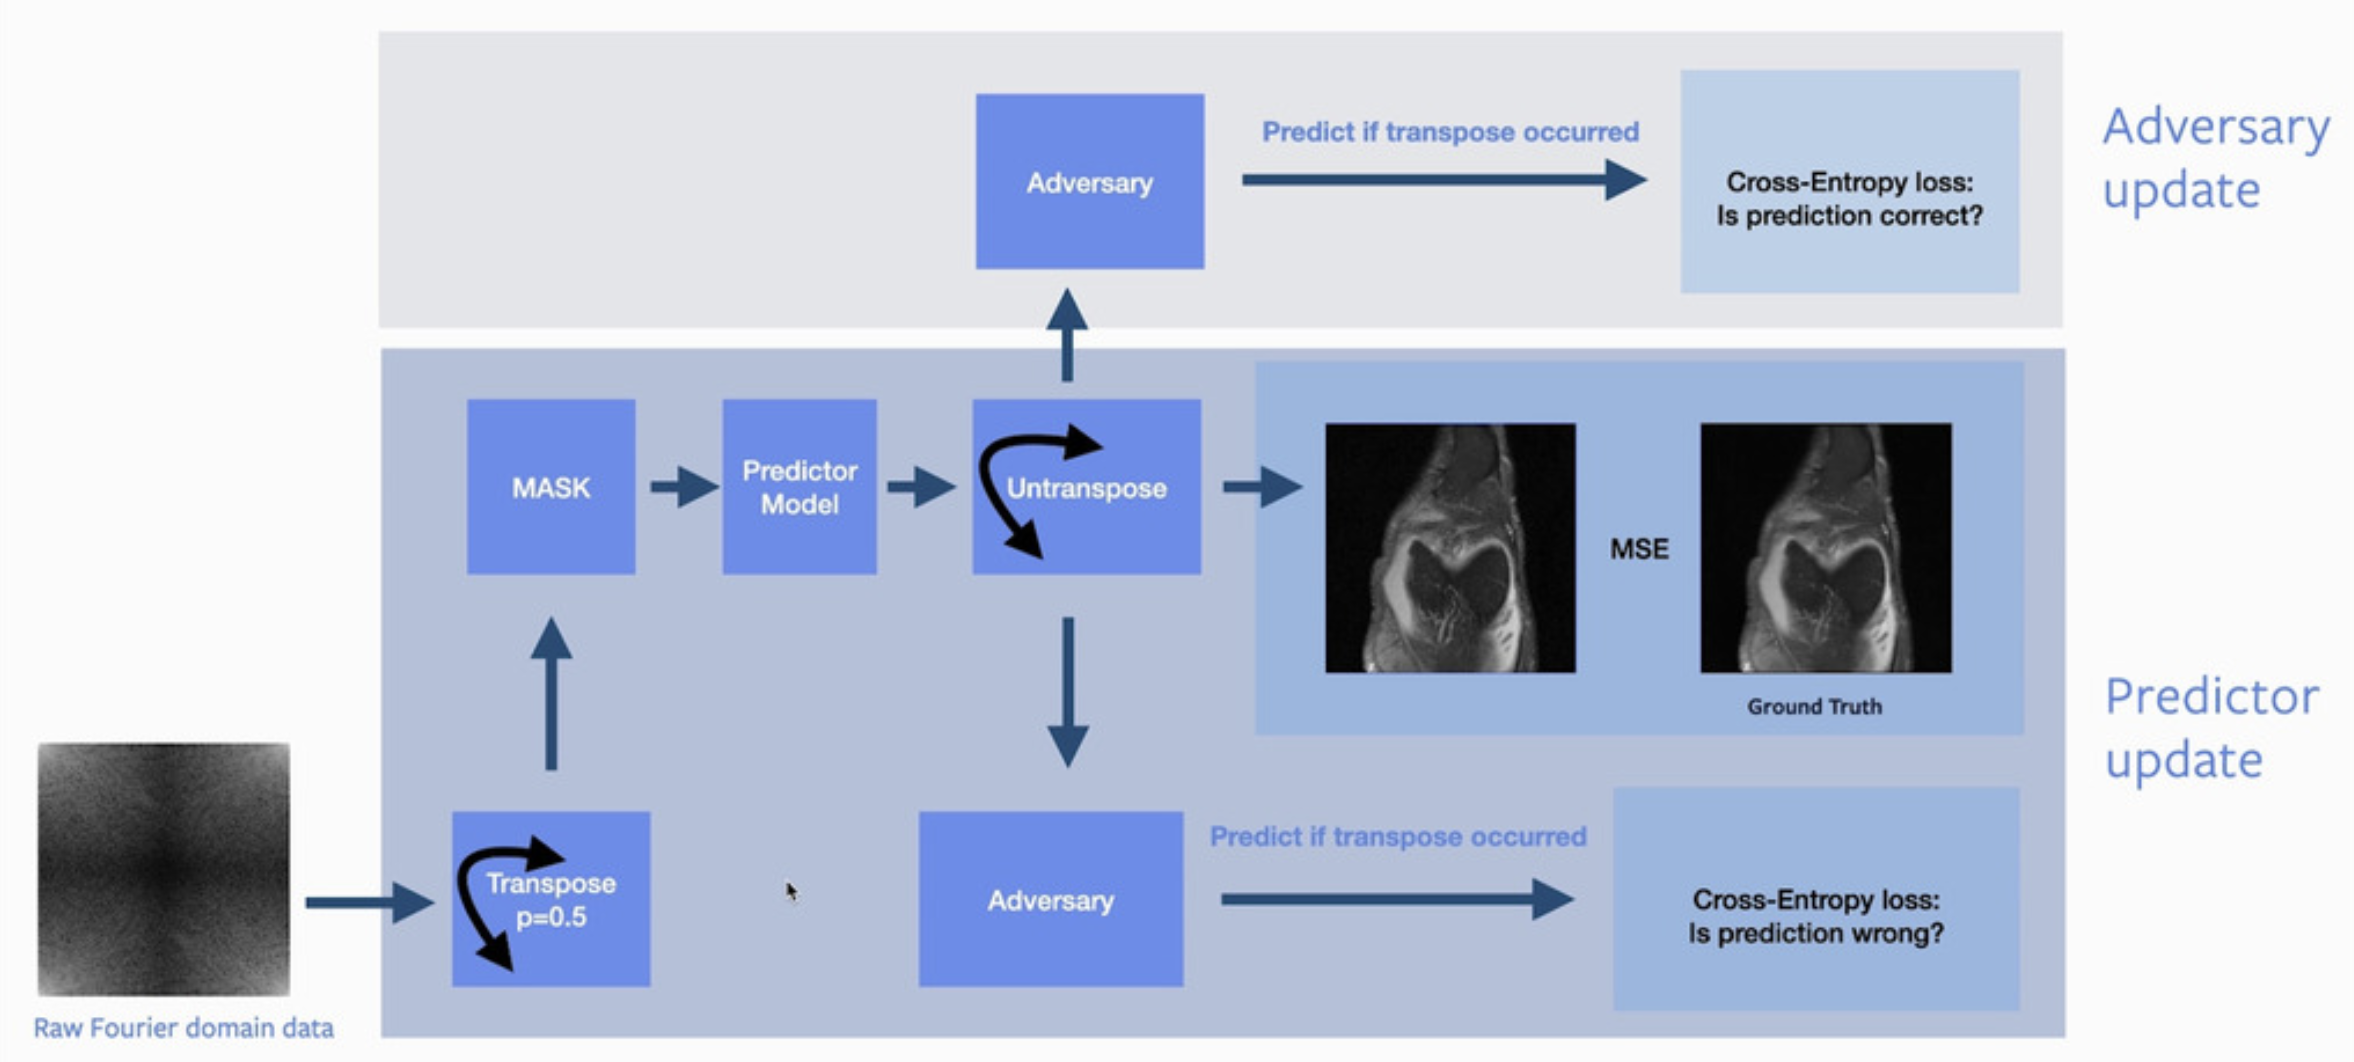
\includegraphics[scale=0.4]{neurips-2020/images/Screenshot 2020-12-15 at 09.34.10.png}
    \caption{Illustration of the full pipeline. Initial raw k-space data can is transposed with $p = 0.5$ and then fed into any reconstruction model. Next, transposed images are reverted back to the normal orientation and together with not transposed ones are fed into a discriminator network. Together with the initial supervised loss, adversarial loss in used to optimize reconstruction model. The proposed system can be trained end-to-end.}
    \label{fig:adversaria_art_removal_pipeline}
\end{figure}

{\bf Results:} the proposed technique produces outputs with little is any banding artefacts (fig. \ref{fig:result_adv_art_removal}).

\begin{figure}[h!]
    \centering
    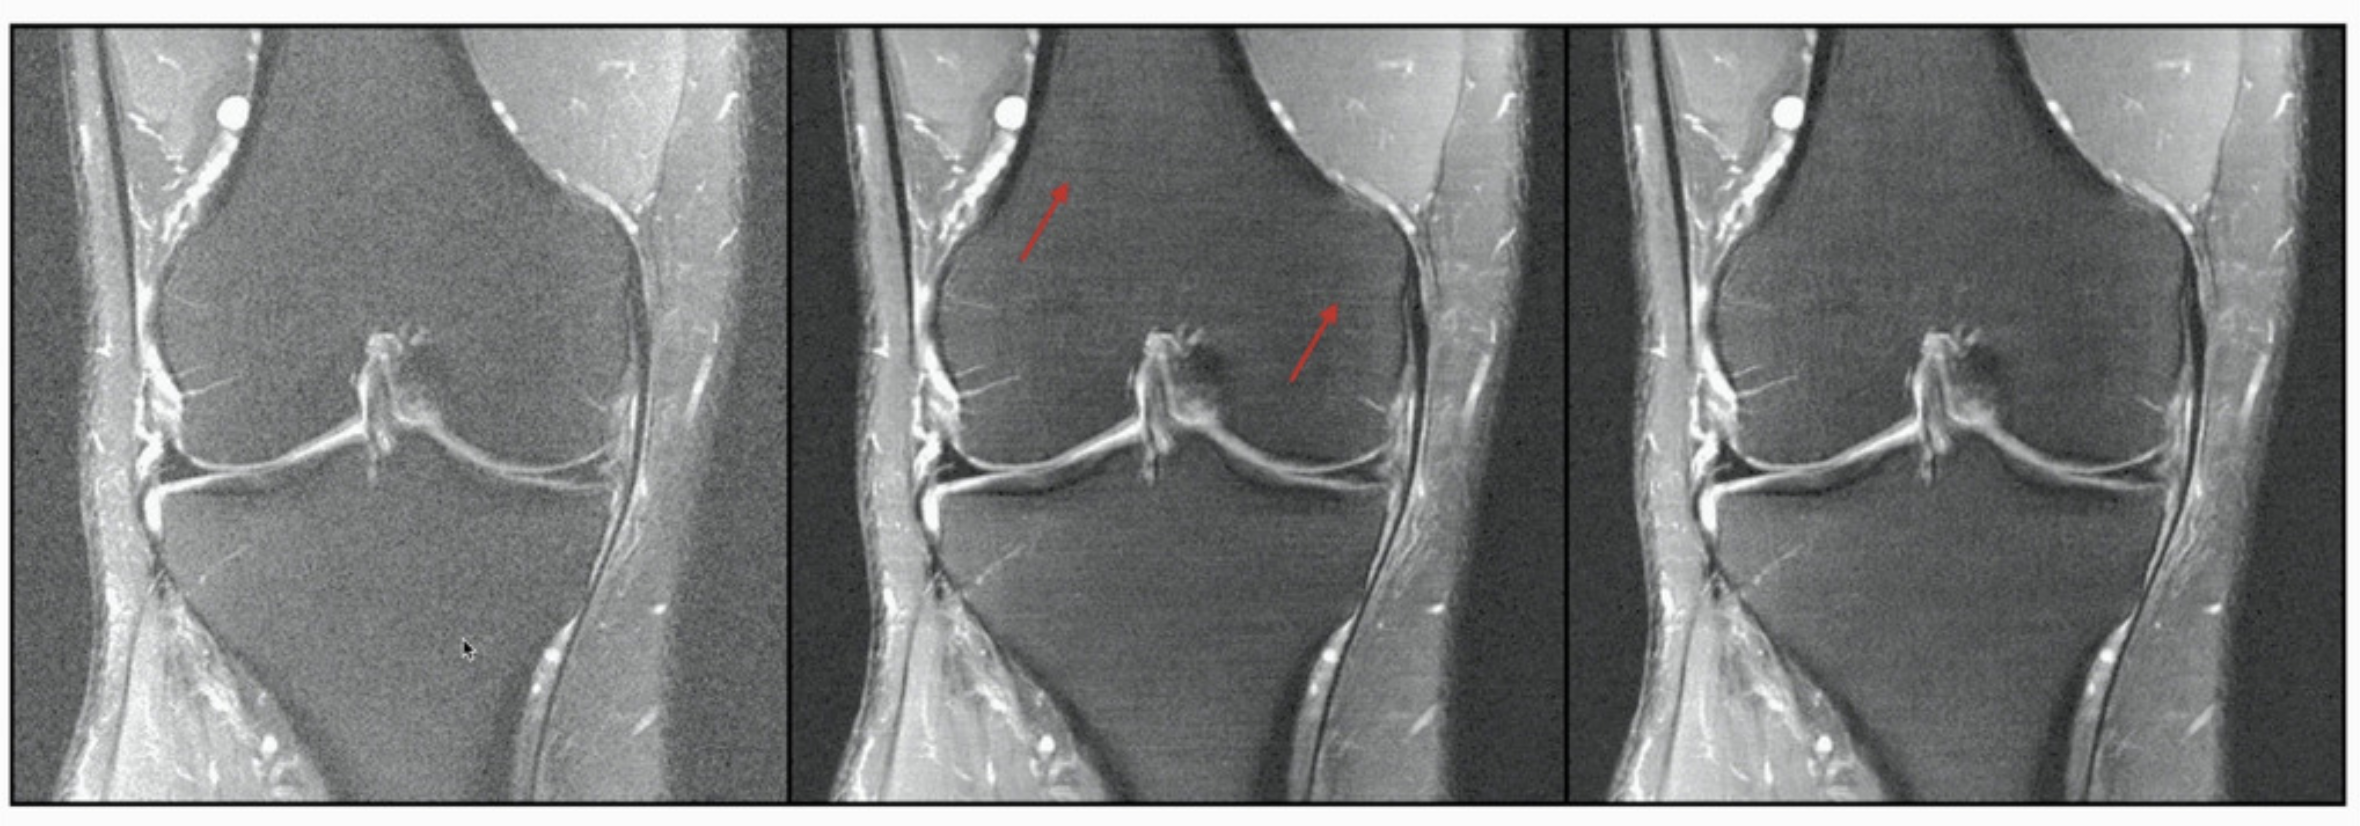
\includegraphics[scale=0.4]{neurips-2020/images/Screenshot 2020-12-15 at 09.45.10.png}
    \caption{Illustration of results from the proposed artefacts removel system. From left to right: fully sampled ground truth image (no artefacts), output of the standard model (artefacts are present), output of the proposed system trained with the adversarial component (less artefacts).}
    \label{fig:result_adv_art_removal}
\end{figure}
